\documentclass[11pt,paper=a4,answers]{exam}
\usepackage{graphicx,lastpage}
\usepackage{upgreek}
\usepackage{hyperref}
\usepackage{amsmath}
\usepackage{enumerate}
\usepackage{censor}
\usepackage{amsmath,amssymb,amsfonts}
\usepackage{tcolorbox}
\usepackage[utf8]{inputenc}
\usepackage{array}
\usepackage{enumitem}

\censorruledepth=-.2ex
\censorruleheight=.1ex
\hyphenpenalty 10000
\usepackage[paperheight=10.5in,paperwidth=8.27in,bindingoffset=0in,left=0.8in,right=1in,
top=0.7in,bottom=1in,headsep=.5\baselineskip]{geometry}
\flushbottom
\usepackage[normalem]{ulem}
\renewcommand\ULthickness{2pt}
\setlength\ULdepth{1.5ex}
\renewcommand{\baselinestretch}{1}
\pagestyle{empty}
\hypersetup{
    colorlinks=true,
    linkcolor=blue,
    filecolor=magenta,      
    urlcolor=blue,
    pdftitle={TOPIC NAME}
    }
\pagestyle{headandfoot}
\headrule

\runningheader{\footnotesize}
{How Do We Virtualize Network Functions?}
\footrule
\footer{\footnotesize}
{\hrule width \textwidth height 1pt \vspace{1mm} Page \thepage\ of \numpages}
{}

\pointsinrightmargin
\pointsdroppedatright
\marksnotpoints
\marginpointname{ \points}
\pointformat{\boldmath\themarginpoints}

\begin{document}

\thispagestyle{empty}

\begin{tcolorbox}[colback=blue!10!white, colframe=gray!20!blue, width=\textwidth, boxrule=0.5mm, arc=0mm, auto outer arc]
    \begin{tabular*}{\textwidth}{@{\extracolsep{\fill}} l r}
        \textbf{CS60203: Design Optimization of Computing Systems} & \textit{\today} \\
    \end{tabular*}
    \begin{center}
        \textbf{\LARGE How Do We Virtualize Network Functions?}
    \end{center}
    \begin{tabular*}{\textwidth}{@{\extracolsep{\fill}} l r}
        \textit{Instructor: Sandip Chakraborty} & \textit{Scribe-By: Sanskar Mittal} \\
    \end{tabular*}
\end{tcolorbox}


\vspace{2mm}

\noindent
\section{Introduction}
We know that network consists of routing which involves forwarding packets from source to destination. Routing can occur within a subnet using switches and routers or between subnets using bridges. However, that's not the only picture in reality ! There's a lot of in-network processing at each point such as node balancing, firewalls, intrusion detection system (IDS), etc. These are called \textbf{Middleboxes} and are part of network management system (NMS). With time, NMS has become more complicated with new applications, devices, policies and threats.

\section{Middleboxes kill Network Performance}
\href{https://dl.acm.org/doi/pdf/10.1145/2377677.2377680}{[Sherry et. al.]} discuss how middlebox infrastructure is expensive, complex to manage, and creates new failure modes for the networks that use them. 
\begin{enumerate}
    \item Middlebox deployment is on par with the number of routers in a network!
    \item It increases both capital expenditure (\textbf{capex}) and operational expenditure (\textbf{opex}) in management
    \item Misconfiguration, Overload and Physical/Electric Failure are most common cause of middlebox failure 
\end{enumerate}

\section{Network Virtualization}
Main idea is to decouple hardware and software instead of having specialised boxes for each of the separate functions.
This reduces capex, enables extensibility and flexible resource allocation. 
\textbf{Virtual Machines} (VMs) can be used to implement network functions.
\begin{itemize}
    \item Application functionalities (NATs, Firewalls, IDS, Proxies)
    \item Network functionalities (Routing algorithms, Forwarding policies)
    \item Security functionalities (Authentication, Authorization, Access control)
\end{itemize}
Even \textbf{lightweight containers} like dockers, kubernetes can be used to implement network functions. They provide all the advantages of virtualization like quick provisioning, scalability, reduced capex and opex, mobility, etc. APIs for communication across the VNFs and across VNFs and hosts has also been standardized (ETSI NFV Release 6, Started 2023).

\newpage
\section{Architecture of 5G system}
\begin{figure}[h]
    \centering
    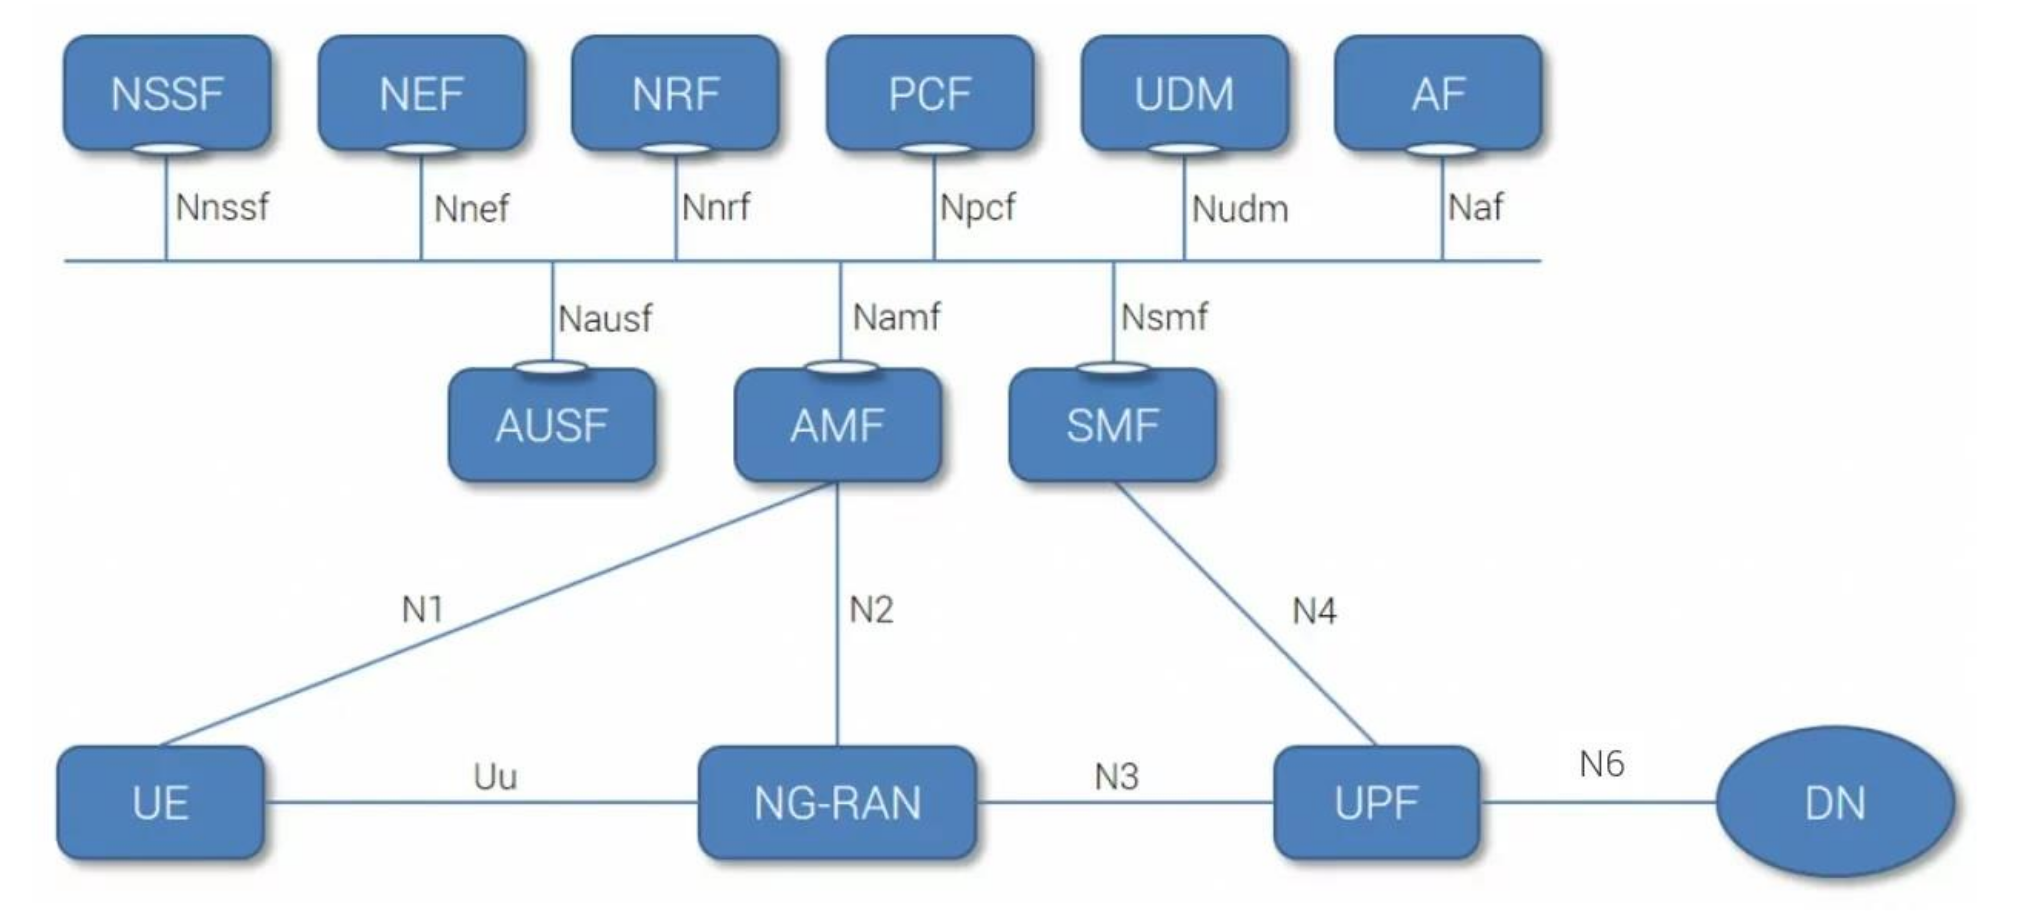
\includegraphics[width=1\textwidth]{Pictures/5G.png}
    \caption{System Architecture for the 5G System (Stage 2)}
    \label{fig:5G_architecture}
\end{figure}

\begin{itemize}
    \item User plane function (\textbf{UPF}) to support forwarding and routing
    \item Access and Mobility Management Function (\textbf{AMF})
    \item Session Management Function (\textbf{SMF})
    \item Policy Control Function (\textbf{PCF})
    \item Authentication Server Function (\textbf{AUSF})
    \item Unified Data Management (\textbf{UDM}) - Authentication and Key Agreement (\textbf{AKA})
    \item Network Exposure Function (\textbf{NEF})
    \item Network Slice Selection Function (\textbf{NSSF})
\end{itemize}

\section{Key NFV Concepts}
\begin{itemize}[leftmargin=*]
    \item \textbf{Network Function(NF):} Functional building block with a well-defined interface and well-defined functional behavior
    \item \textbf{Virtualized Network Function (VNF):} Software implementation of NF that can be deployed in a virtualized infrastructure
    \item \textbf{VNF Set:} Connectivity between VNFs is not specified, e.g., residential gateways
\end{itemize}

\newpage
\begin{figure}[h]
    \centering
    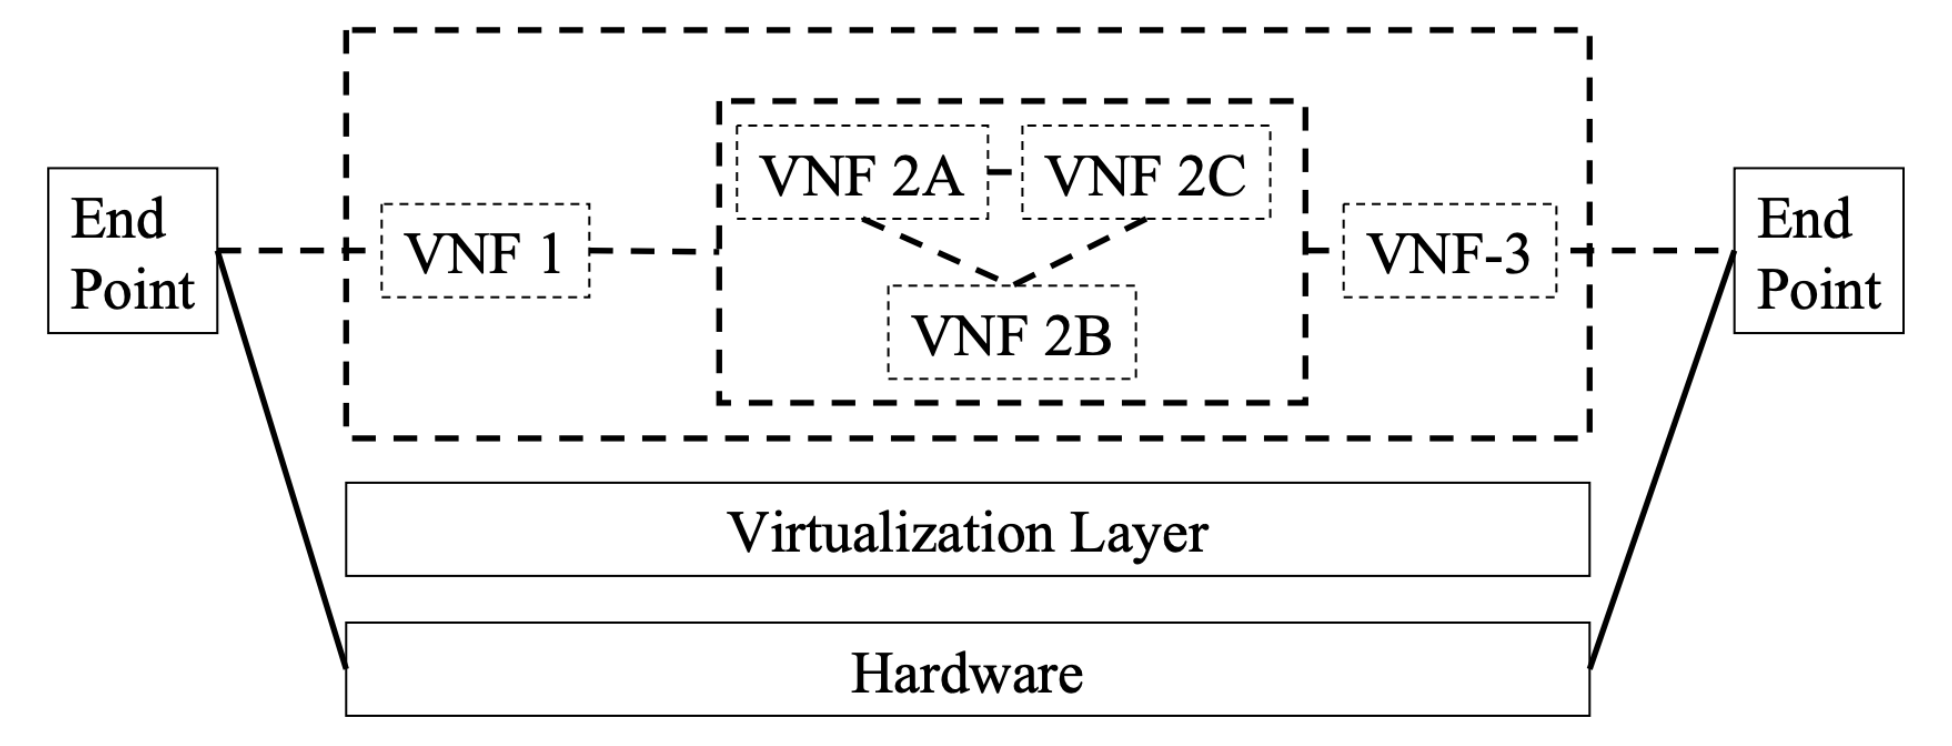
\includegraphics[width=1\textwidth]{Pictures/NFG.png}
    \caption{Network Forwarding Graph}
    \label{fig:NFG}
\end{figure}

\begin{itemize}[leftmargin=*]
    \item \textbf{VNF Forwarding Graph:} Service chain when network connectivity order is important, e.g., firewall, NAT, load balancer
    \item \textbf{NFV Infrastructure:} Hardware and software required to deploy, mange and execute VNFs including computation, networking, and storage
    \item \textbf{NFVI Point of Presence (PoP):} Location of NFVI
    \item \textbf{NFVI-PoP Network:} Internal network
    \item \textbf{Transport Network:} Network connecting a PoP to other PoPs or external networks
    \item \textbf{VNF Manager:} VNF lifecycle management e.g., instantiation, update, scaling, query, monitoring, fault diagnosis, healing, termination
    \item \textbf{Virtualized Infrastructure Manager:} Management of computing, storage, network, software resources
    \item \textbf{Network Service:} A composition of network functions and defined by its functional and behavioral specification
    \item \textbf{NFV Service:} A network service using NFs with at least one VNF.
    \item \textbf{User Service:} Services offered to end users/customers/subscribers.
    \item \textbf{Deployment Behavior:} NFVI resources that a VNF requires, e.g., Number of VMs, memory, disk, images, bandwidth, latency
    \item \textbf{Operational Behavior:} VNF instance topology and lifecycle operations, e.g., start, stop, pause, migration, etc.
    \item \textbf{VNF Descriptor:} Deployment behavior + Operational behavior
    \item \textbf{NFV Orchestrator:} Automates the deployment, operation, management, coordination of VNFs and NFVI.
\end{itemize}

\newpage
\section{NFV Reference Points}

\begin{figure}[h]
    \centering
    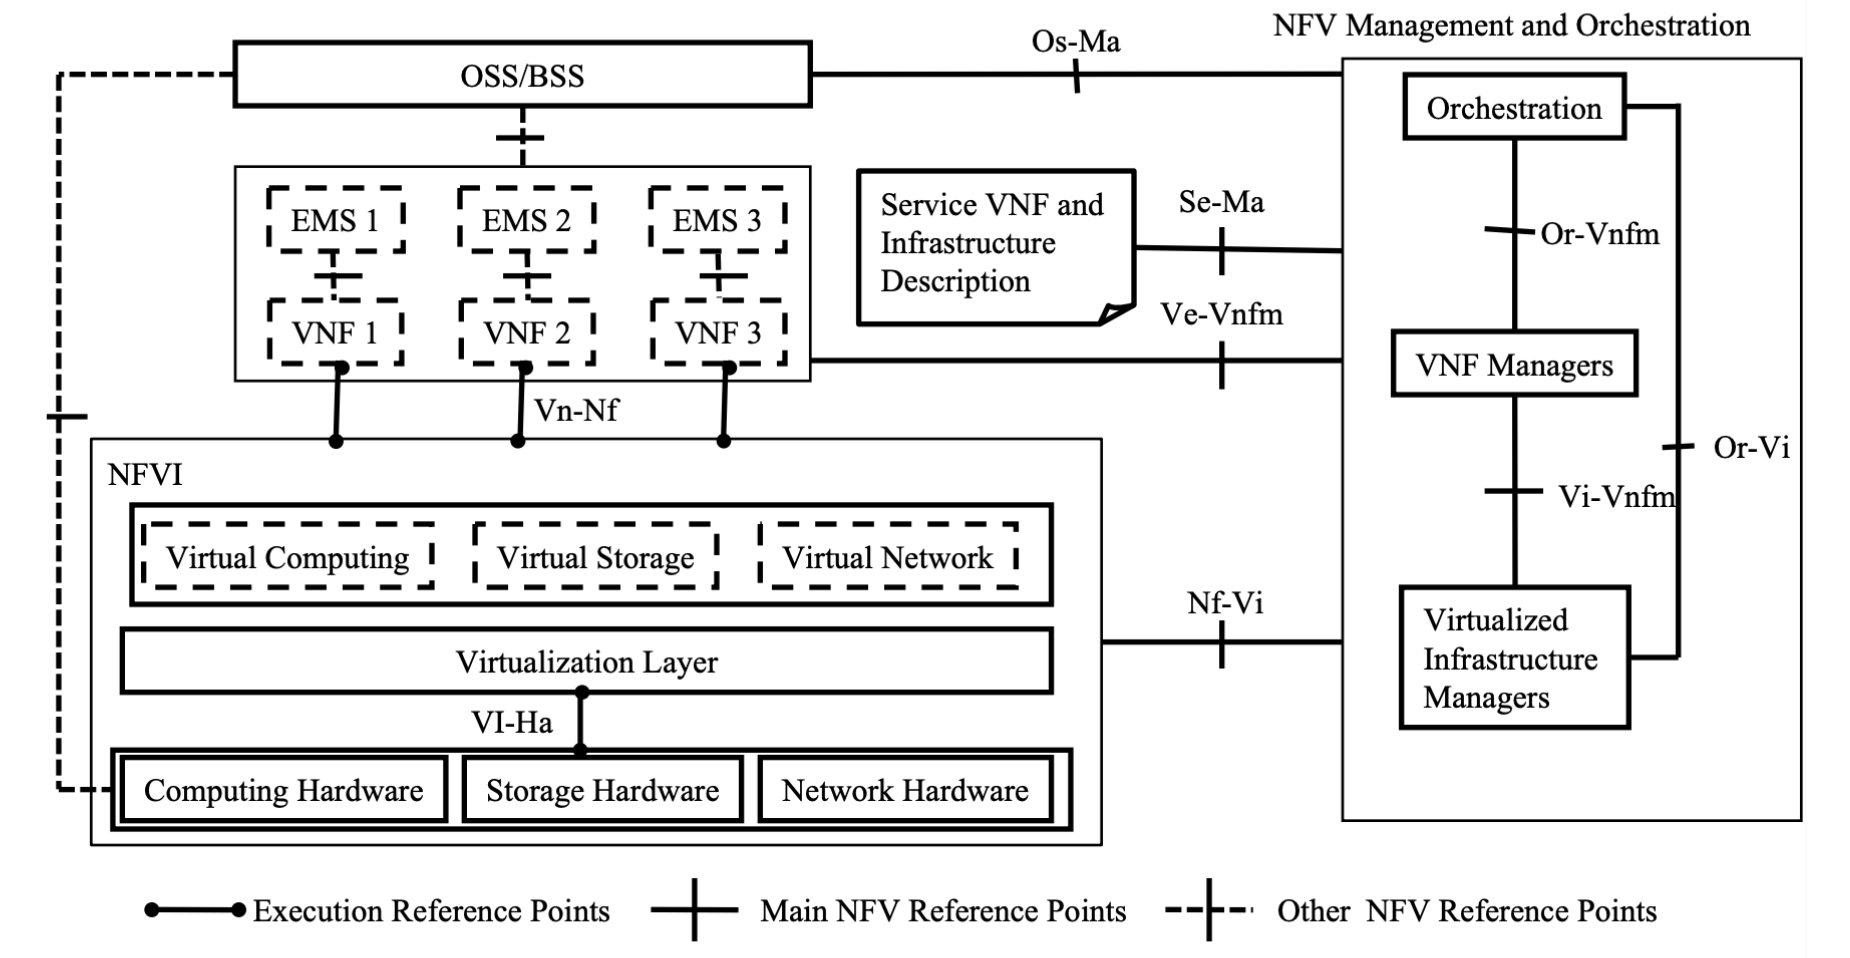
\includegraphics[width=1\textwidth]{Pictures/NFV_architecture.png}
    \caption{NFV Architecture}
    \label{fig:NFV_Architecture}
\end{figure}

\begin{itemize}[leftmargin=*]
    \item \textbf{VI-Ha:} Virtualization Layer-Hardware Resources
    \item \textbf{Vn-Nf:} VNF – NFVI
    \item \textbf{Or-Vnfm:} Orchestrator – VNF Manager
    \item \textbf{Vi-Vnfm:} Virtualized Infrastructure Manager – VNF Manager
    \item \textbf{Or-Vi:} Orchestrator – Virtualized Infrastructure Manager
    \item \textbf{Nf-Vi:} NFVI-Virtualized Infrastructure Manager
    \item \textbf{Os-Ma:} Operation Support System (OSS)/Business Support Systems (BSS) – NFV Management and
    Orchestration
    \item  \textbf{Ve-Vnfm:} VNF/ Element Management System (EMS) – VNF Manager
    \item \textbf{Se-Ma:} Service, VNF and Infrastructure Description – NFV Management and Orchestration
\end{itemize}

\section{Summary}
In-network packet processing is expensive, especially for middleboxes. Virtualization at the network core makes management flexible, reducing capex and opex. It is the key behind 5G/6G network core. It also has flexible APIs, network slicing (creating multiple virtual networks on top of a shared
physical infrastructure) and app stack. Thus, it provides innovation and management optimzation over classical protocol stack.


\end{document}